\documentclass{summarysheet}

\begin{document}


\maketitle{3}{The Electric Field II}

\begin{multicols}{2}

\begin{topicbox}{The Electric Field Concept}

\noindent The electric field is an alteration of space surrounding charge. It is created by source charge and exerts an electric force on other charge.

The electric field is defined by its effect on a \emph{test charge} $q$:
\[
\vec{E} = \frac{\vec{F}_\text{on $q$}}{q}.
\]

The units of the electric field are N/C or V/m.

\textbf{The electric field exerts a force on charge.}  For a point charge $q$, the force is given by
\begin{teqbox}
\[
\vec{F} = q\vec{E}.
\]
\end{teqbox}

\end{topicbox}


\begin{topicbox}{Electric Field of Point Charges}

\noindent A single point charge $q$ generates an electric field given by
\[
\vec{E} = \frac{1}{4\pi \varepsilon_0 } \frac{q}{r^2} \, \hat{r}.
\]
The electric field points \emph{away} from positive charge and \emph{toward} negative charge.

Multiple point charges $q_i$ generate an electric field given by the principle of superposition -- we just add up each individual electric field:
\begin{teqbox}
\[
\vec{E}_\text{net} = \sum_i \frac{1}{4\pi \varepsilon_0 } \frac{q_i}{r_i^2} \, \hat{r}_i.
\]
\end{teqbox}

\end{topicbox}


\begin{topicbox}{Charge Densities}

\noindent For extended charged objects, we can define three charge densities depending on the shape:
\begin{teqbox}
\begin{itemize}
\item Linear charge density (C/m):  $\lambda = Q/L$.
\item Surface charge density (C/m$^2$): $\eta = Q/A$.
\item Volume charge density (C/m$^3$): $\rho = Q/V$.
\end{itemize}
\end{teqbox}

\end{topicbox}




\begin{topicbox}{Electric Dipoles}

\begin{multicols}{2}

An electric dipole is formed when two equal but opposite charges are very close together.  They can be \emph{permanent} (e.g., water molecules) or \emph{induced}.  

The electric field far from a dipole is
\[
\vec{E} \approx \frac{1}{4\pi \epsilon_0} \frac{2\vec{p}}{r^3}
\]
for points on the axis of the dipole or
\[
\vec{E} \approx -\frac{1}{4\pi \epsilon_0} \frac{\vec{p}}{r^3}
\]
for points on the bisecting line.

In a \emph{uniform} external field $\vec{E}_\text{ext}$, dipoles feel a torque
\[
\vec{\tau} = \vec{p} \times \vec{E}_\text{ext}.
\]
In a \emph{nonuniform} external field, dipoles also feel a net force toward the direction of stongest electric field.

\begin{center}
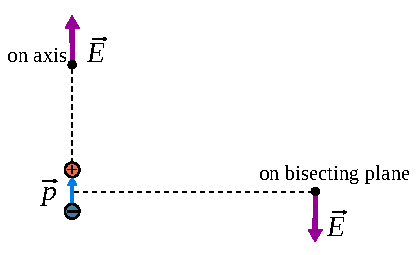
\includegraphics[scale=0.7]{fig_dipole1.pdf}
\end{center}

\begin{center}
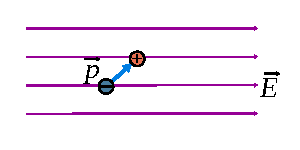
\includegraphics[scale=0.7]{fig_dipole2.pdf}
\end{center}


\end{multicols}

\end{topicbox}




\begin{topicbox}{Continuous Charge Distributions}

\noindent If an object contains many excess electrons or protons we can consider the charge to be continuous rather than at a point.  Some common charge distributions are:
\begin{multicols}{2}
\begin{itemize}
\item Infinite line of charge, charge density $\lambda$
\[
E = \frac{1}{4\pi \epsilon_0} \frac{2|\lambda|}{r} 
\]
\item Ring of charge, along axis, total charge $Q$, radius $R$
\[
E =  \frac{1}{4\pi \epsilon_0} \frac{zQ}{(z^2 + R^2)^{3/2}}
\]
\item Disk of charge, surface charge density $\eta$, radius $R$
\[
E = \frac{ \eta}{2\epsilon_0} \left( 1 - \frac{z}{\sqrt{z^2 + R^2}} \right)
\]
\item Plane of charge, surface charge density $\eta$
\[
E = \frac{\eta}{2\epsilon_0}
\]
\item Sphere of charge, total charge $Q$, radius $R$
\[
E = \frac{1}{4\pi \epsilon_0} \frac{Q}{r^2}
\]
\end{itemize}

\begin{center}

\includegraphics[scale=0.7]{fig_continuous.pdf}
\end{center}

\end{multicols}

\end{topicbox}

\begin{topicbox}{The Parallel Plate Capacitor}

The electric field outside an ideal capacitor is zero; inside it is uniform and points from the positive plate to the negative:
\begin{teqbox}
\[
E = \frac{Q}{\epsilon_0 A}.
\]
\end{teqbox}

\begin{center}
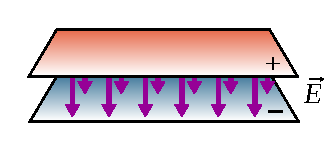
\includegraphics[scale=0.8]{fig_capacitor.pdf}
\end{center}

\end{topicbox}






\end{multicols}


\makebanner{Electricity and Magnetism}

\end{document}



